\newpage
\section{Экспериментальная установка}
Принципиальная схема релаксометра ЯМР приведена на рис. \ref{fig:installation}

\begin{figure}[h]
	\centering
	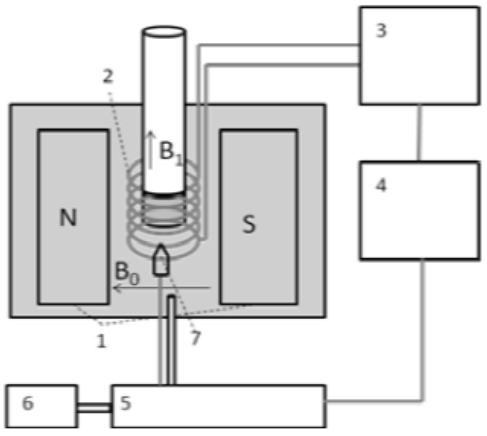
\includegraphics[width=0.6\linewidth]{Installation}
	\caption{Принципиальная схема: \textbf{1} -- постоянный магнит; \textbf{2} -- приемопередающая катушка; \textbf{3} -- генератор импульсов и приемник излучения; \textbf{4} -- компьютер; \textbf{5} -- система термостатирования образца; \textbf{6} -- воздушный компрессор; \textbf{7} -- термопара}
	\label{fig:installation}
\end{figure}

Основной частью ЯМР-релаксометра является магнит (\textbf{1} на рис. \ref{fig:installation}), создающий постоянное магнитное поле напряженностью $ \vec{B}_0 $. 

Переменное магнитное поле, перпендикулярное постоянному магнитному полю, создается при помощи катушки индуктивности, вдоль оси которой располагается пробирка с исследуемым образцом. Параллельно катушке включен конденсатор так, что образованный радиочастотный контур настроен на резонансную ларморовскую частоту.

Для созданя импульсов переменного поля катушка \textbf{2} соединяется с радиочастотным генератором, расположенным в \textbf{3}. Слабый сигнал ЯМР предварительно усиливается, затем поступает в блок управляющей электроники, где и производится его детектирование. При этом следует учитывать наличие переходных процессов в приемном контуре и усилителе, из-за которых у приемника существует т.н. <<мертвое время>> порядка 100 нс, необходимое для переключения в режим приема и усиления слабого сигнала намагниченности после периода генерации мощных импульсов.

\subsection{Ход работы}
\begin{enumerate}
	\item Получение результатов ЯМР в программе
	\item Изучение общего вида спектра при различных рабочих частотах
	\item Определение химического сдвига и относительной интенсивности составляющих спектра
	\item Исследование тонкой структуры, выводы и оценка неоднородности поля 
\end{enumerate}
